\documentclass[conference]{IEEEtran}
\usepackage[utf8]{inputenc}
\usepackage{graphicx}
\usepackage{amsmath}
\usepackage{cite}
\usepackage{float}

\title{Evaluación Comparativa entre un Modelo Residual Ligero y ResNet50 para Clasificación Histopatológica de Cáncer Pulmonar}

\author{
  \IEEEauthorblockN{Joel Luis Ibaceta Canchaya}
  \IEEEauthorblockA{
    \textit{Universidad Nacional de Ingeniería} \\
    joel.ibaceta.c@uni.pe
  }
  \and
  \IEEEauthorblockN{Marco Antonio Barrera Ninamango}
  \IEEEauthorblockA{
    \textit{Universidad Nacional de Ingeniería} \\
    marco.barrera.n@uni.pe
  }
  \and
  \IEEEauthorblockN{Jesus Gianpierre Campos Cardenas}
  \IEEEauthorblockA{
    \textit{Universidad Nacional de Ingeniería} \\
    j.campos.c@uni.pe
  }
}


\begin{document}

\maketitle

\begin{abstract}
Este estudio explora el uso de redes neuronales convolucionales residuales para la clasificación de imágenes histopatológicas de cáncer de pulmón, comparando dos enfoques: un modelo ligero personalizado, \textit{ResNetLung}, basado en ResNet-18, y una red profunda preentrenada, ResNet50. Ambos modelos fueron evaluados sobre un subconjunto del dataset LC25000, centrado en adenocarcinoma, carcinoma de células escamosas y tejido sano. \textit{ResNetLung}, entrenado desde cero por 10 épocas, logró una precisión del 96\% y un macro F1-score de 0.96, superando a ResNet50, que alcanzó un 88.6\% de precisión tras 30 épocas de ajuste fino. Los resultados evidencian que, en dominios visuales específicos como la histopatología, modelos más simples y alineados al problema pueden superar a arquitecturas más complejas, brindando además ventajas en eficiencia computacional y estabilidad. Este trabajo resalta el potencial de soluciones adaptadas al dominio para asistir en el diagnóstico médico automatizado.
\end{abstract}

\section{Introducci\'on}

El cáncer de pulmón es una de las principales causas de mortalidad a nivel mundial. El diagnóstico temprano mediante análisis histopatológico es esencial para mejorar el pronóstico, pero requiere tiempo, recursos especializados y experiencia médica considerable. La automatización de esta tarea mediante técnicas de inteligencia artificial puede acelerar y estandarizar la detección de patrones patológicos.

En este trabajo se propone un modelo convolucional residual, denominado \textit{ResNetLung}, implementado desde cero con una arquitectura tipo ResNet-18 para clasificar imágenes histológicas de tejido pulmonar. Además, se incluye una prueba comparativa con una red profunda preentrenada ResNet50 \cite{he2016resnet}, permitiendo evaluar el desempeño entre un modelo ligero personalizado y uno de mayor profundidad ampliamente utilizado.
\section{Metodolog\'ia}

\section{Dataset}

Se utilizó el conjunto de datos LC25000, del cual se seleccionaron únicamente las clases relacionadas al pulmón: adenocarcinoma (\texttt{lung\_aca}), tejido sano (\texttt{lung\_n}) y carcinoma de células escamosas (\texttt{lung\_scc}). Cada clase contiene imágenes histopatológicas teñidas con hematoxilina y eosina (H\&E), capturadas con aumentos microscópicos homogéneos.

La Figura~\ref{fig:dataset} muestra una selección de imágenes representativas para cada clase, donde se pueden observar diferencias visuales en la morfología celular y la estructura del tejido.

\begin{figure}[H]
\centering
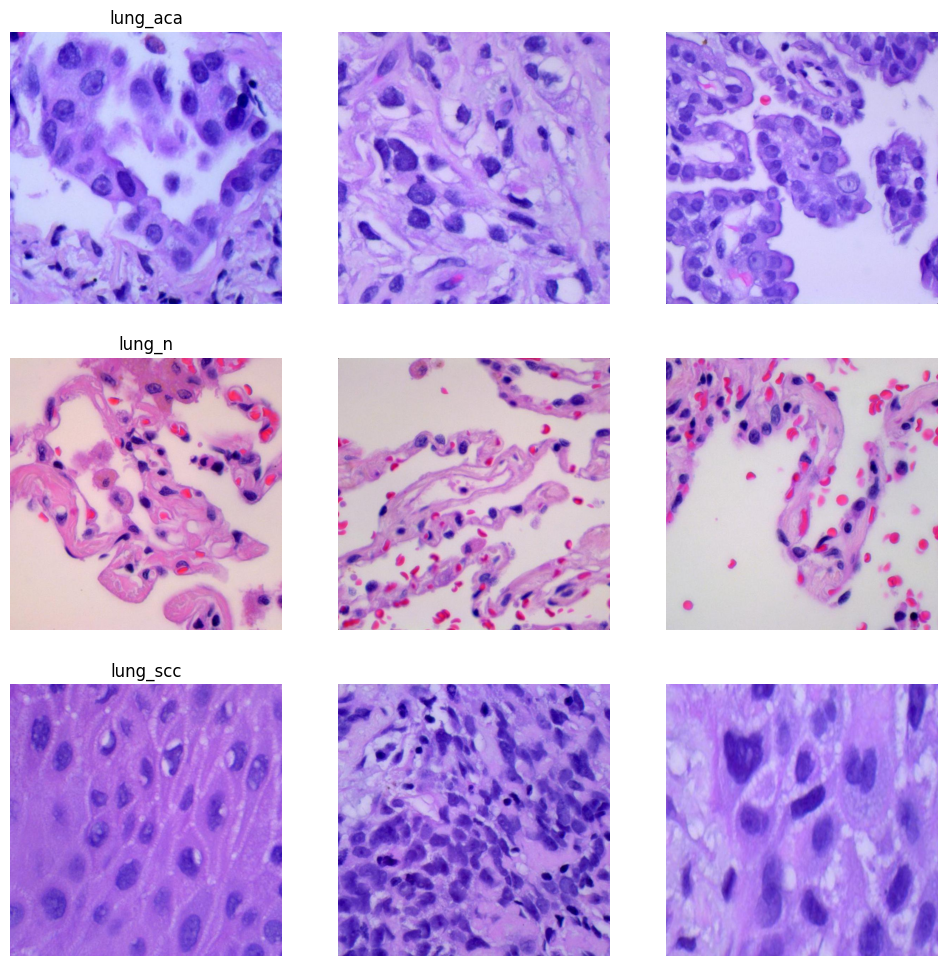
\includegraphics[width=0.48\textwidth]{figs/dataset_exploration.png}
\caption{Ejemplos de imágenes histopatológicas por clase: adenocarcinoma (arriba), tejido sano (medio), y carcinoma escamoso (abajo).}
\label{fig:dataset}
\end{figure}

\subsection{Arquitectura del Modelo}

Se compararon dos enfoques arquitectónicos para la clasificación de imágenes histopatológicas de cáncer de pulmón. El primero, que denominamos \textit{ResNetLung}, corresponde a una red convolucional residual ligera, implementada desde cero con una configuración equivalente a ResNet-18. Esta red está compuesta por una capa convolucional inicial, cuatro bloques residuales organizados en la secuencia [2,2,2,2], una capa de \textit{pooling} global y una capa densa final. El diseño prioriza la eficiencia computacional sin sacrificar capacidad expresiva.

\begin{figure}[H]
\centering
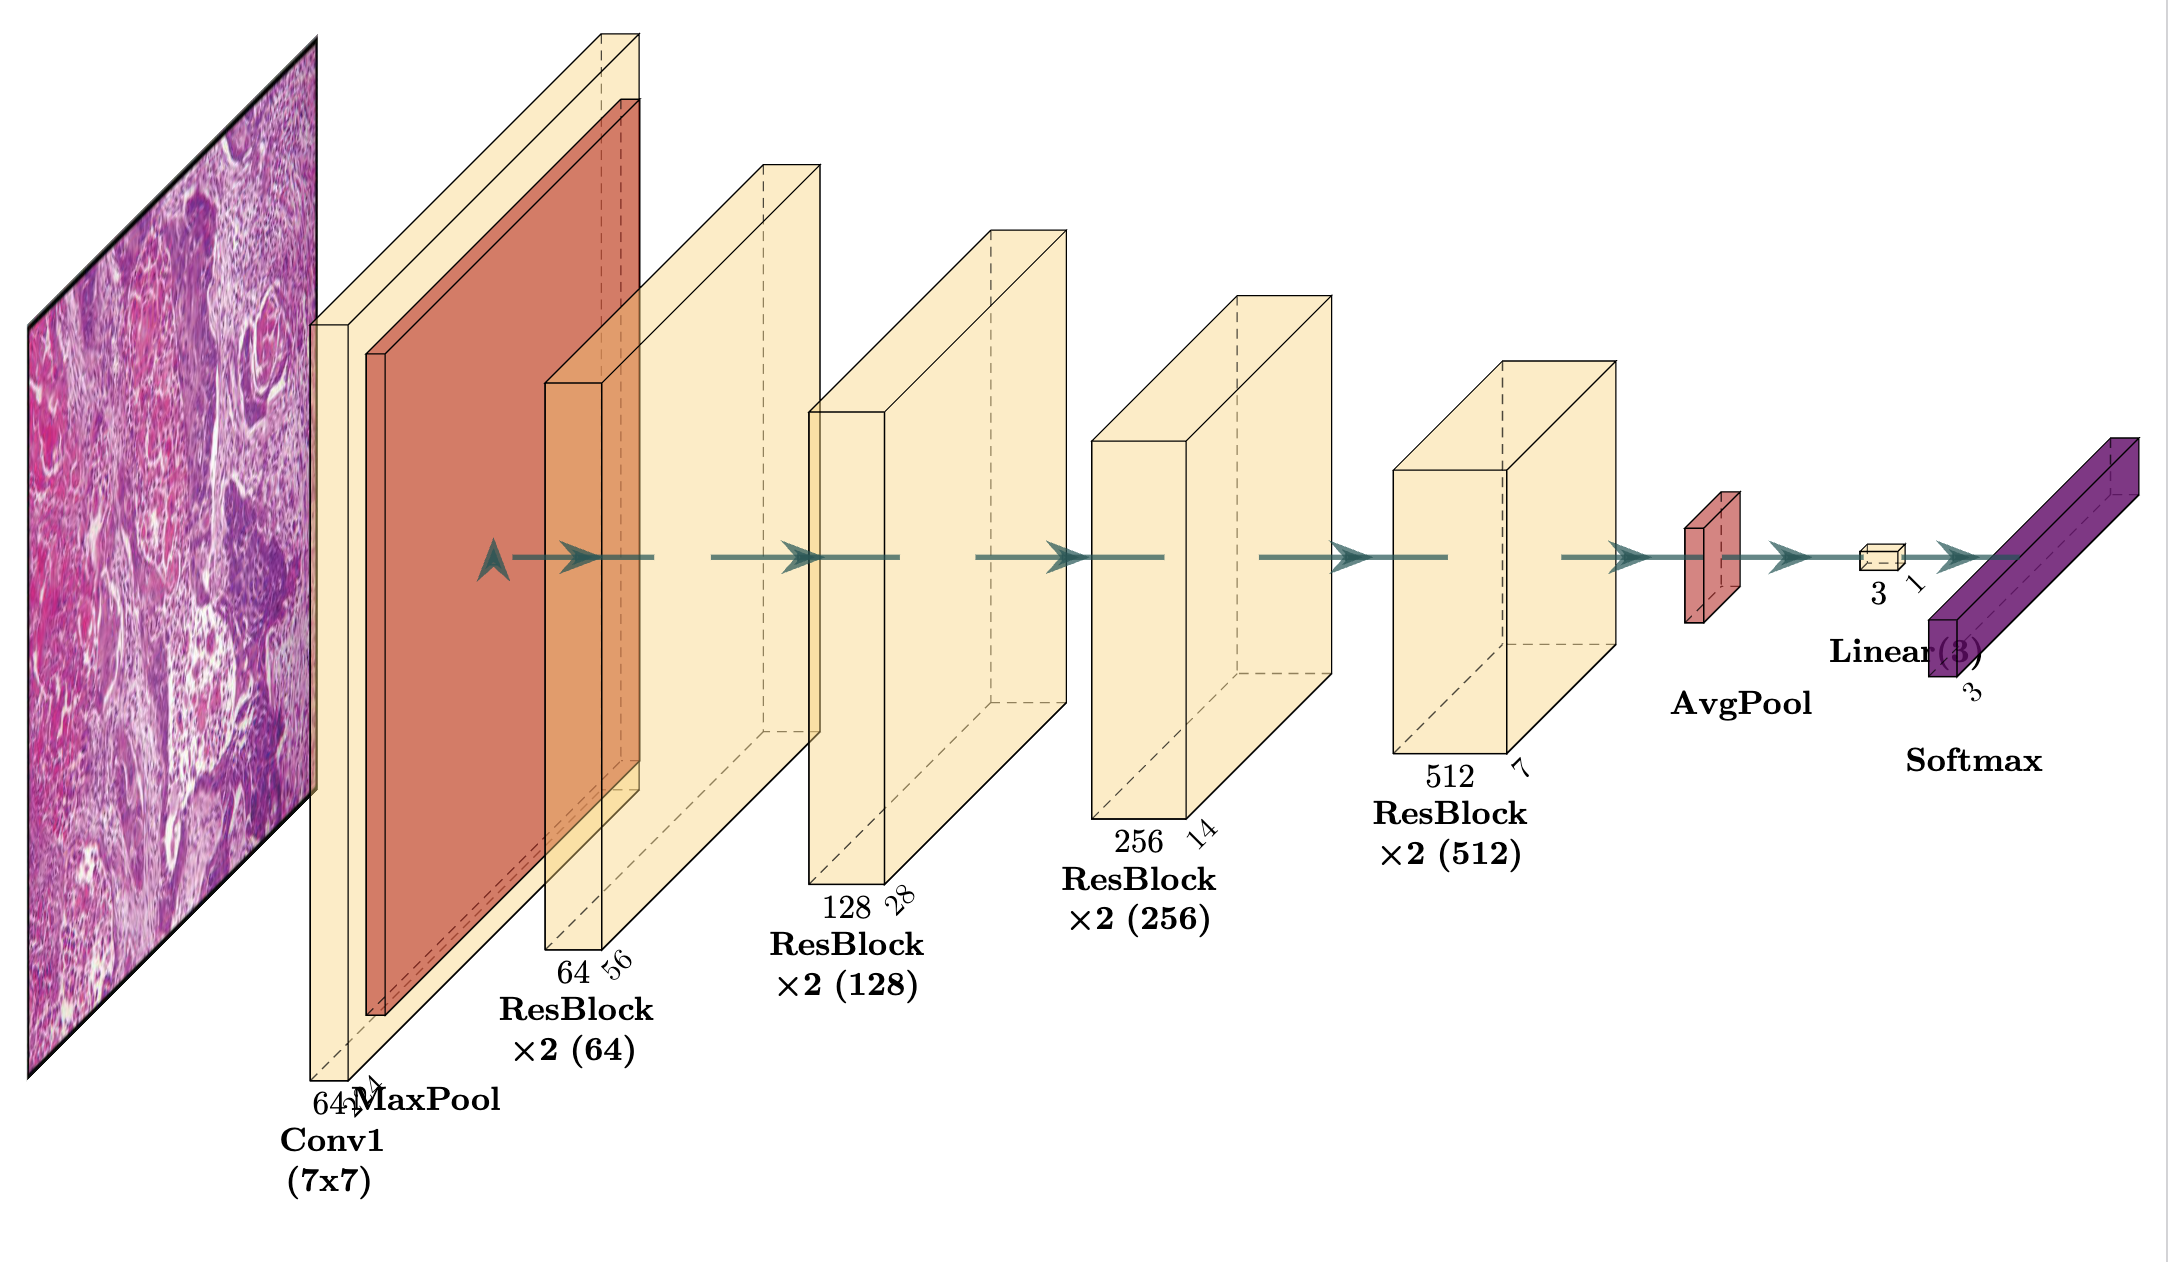
\includegraphics[width=0.48\textwidth]{figs/resnetlung_architecture.png}
\caption{Arquitectura de la red \textit{ResNetLung}, con bloques residuales organizados en cuatro etapas y salida para tres clases.}
\label{fig:architecture}
\end{figure}

El segundo enfoque utiliza una arquitectura ResNet50 \cite{he2016resnet}, considerablemente más profunda, preentrenada sobre el conjunto ImageNet y adaptada a la tarea mediante aprendizaje transferido. Se removió la cabeza clasificadora original y se añadió una nueva capa densa con tres salidas y activación \texttt{softmax}. Las capas convolucionales del modelo base se mantuvieron congeladas durante el entrenamiento.

\begin{figure}[H]
\centering
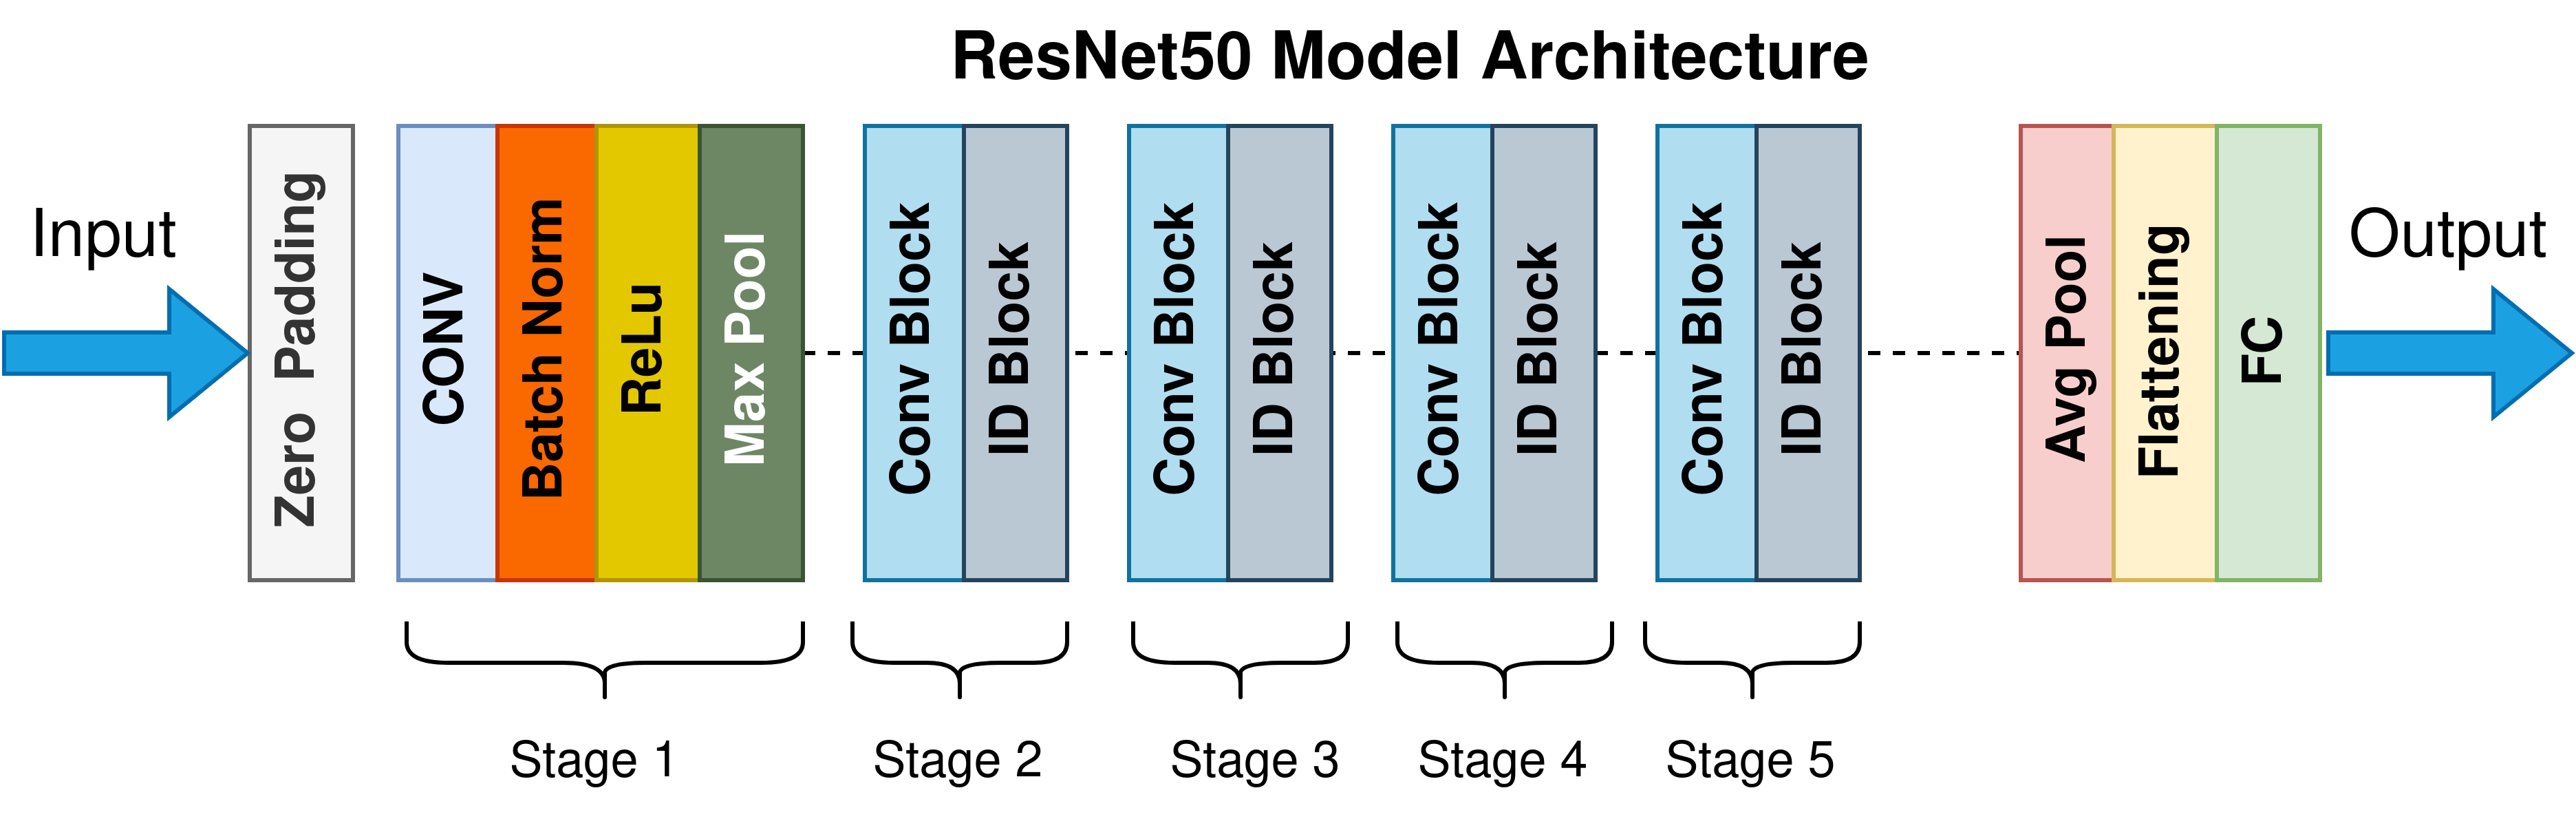
\includegraphics[width=0.48\textwidth]{figs/restnet50.png}
\caption{Arquitectura interna de ResNet50, compuesta por una capa inicial convolucional y cinco etapas residuales con bloques de convolución (Conv Block) y de identidad (ID Block), seguidas de un clasificador denso.}
\label{fig:resnet50}
\end{figure}


\subsection{Justificaci\'on de ResNet-18}
La elecci\'on de ResNet-18 se fundamenta en su equilibrio entre profundidad y eficiencia computacional. Estudios previos demuestran su eficacia en tareas m\'edicas similares. En \cite{xu2024resnet} se us\'o ResNet-18 para clasificaci\'on citol\'ogica respiratoria con buenos resultados. En \cite{wang2024pirads} se utiliz\'o exitosamente para clasificaci\'on de lesiones prost\'aticas.

\section{Entrenamiento}

Se entrenaron por separado dos modelos para la clasificación multiclase de imágenes histopatológicas: \textit{ResNetLung}, diseñado desde cero, y \textit{ResNet50}, un modelo profundo preentrenado. A continuación, se detalla el proceso de entrenamiento de cada uno.

\hspace{0.5cm}

\subsubsection{Entrenamiento de \textit{ResNetLung}}

El modelo \textit{ResNetLung} fue entrenado desde cero durante 10 épocas, utilizando el optimizador Adam con una tasa de aprendizaje inicial de $0.001$ y la función de pérdida \texttt{CrossEntropyLoss}. Todos los pesos de la red fueron inicializados aleatoriamente y optimizados durante el entrenamiento. El proceso se realizó en un sistema macOS con soporte para \texttt{MPS} (Metal Performance Shaders).

La Tabla~\ref{tab:epochacc} muestra la evolución del desempeño del modelo a lo largo de las épocas. Se observa una disminución progresiva de la pérdida, desde $0.3668$ en la primera época hasta $0.1136$ en la última, acompañada de un incremento sostenido en la exactitud, alcanzando un valor final del $95.61\%$.

\begin{table}[ht]
\centering
\caption{Evolución del desempeño de \textit{ResNetLung} por época}
\begin{tabular}{|c|c|c|}
\hline
\textbf{Época} & \textbf{Loss} & \textbf{Accuracy} \\
\hline
1 & 0.3668 & 85.62\% \\
2 & 0.2530 & 89.48\% \\
3 & 0.1953 & 91.87\% \\
4 & 0.1860 & 92.57\% \\
5 & 0.1841 & 92.73\% \\
6 & 0.1511 & 94.03\% \\
7 & 0.1383 & 94.25\% \\
8 & 0.1284 & 94.93\% \\
9 & 0.1269 & 94.89\% \\
10 & \textbf{0.1136} & \textbf{95.61\%} \\
\hline
\end{tabular}
\label{tab:epochacc}
\end{table}

El reporte de clasificación fue el siguiente:

\begin{table}[ht]
\centering
\caption{Reporte de clasificación del modelo \textit{ResNetLung} sobre el conjunto de prueba}
\begin{tabular}{|l|c|c|c|c|}
\hline
\textbf{Clase} & \textbf{Precisión} & \textbf{Recall} & \textbf{F1-score} & \textbf{Soporte} \\
\hline
lung\_aca      & 1.00 & 0.87 & 0.93 & 958 \\
lung\_n        & 1.00 & 1.00 & 1.00 & 1016 \\
lung\_scc      & 0.89 & 1.00 & 0.94 & 1026 \\
\hline
\textbf{Accuracy} & \multicolumn{4}{c|}{0.96 (3000 imágenes)} \\
\textbf{Macro avg} & 0.96 & 0.96 & 0.96 & 3000 \\
\textbf{Weighted avg} & 0.96 & 0.96 & 0.96 & 3000 \\
\hline
\end{tabular}
\label{tab:clasresnetlung}
\end{table}

La Figura~\ref{fig:confmatrix} presenta la matriz de confusión obtenida tras evaluar el modelo sobre el conjunto de prueba. El clasificador muestra un rendimiento robusto en las tres clases analizadas: adenocarcinoma pulmonar (\texttt{lung\_aca}), tejido pulmonar sano (\texttt{lung\_n}) y carcinoma escamoso pulmonar (\texttt{lung\_scc}).

\begin{figure}[H]
\centering
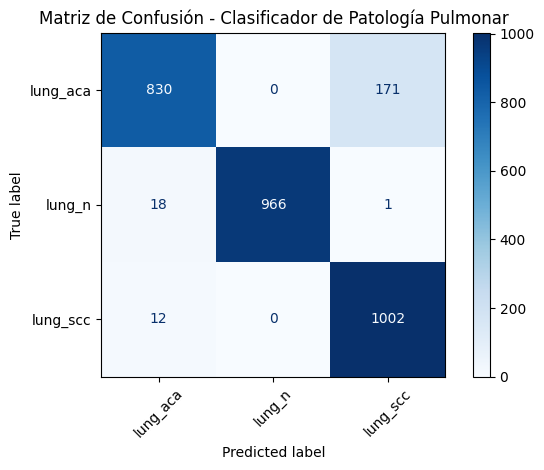
\includegraphics[width=0.45\textwidth]{figs/confusion_matrix.png}
\caption{Matriz de confusión del modelo ResNetLung sobre el conjunto de prueba.}
\label{fig:confmatrix}
\end{figure}

\subsubsection{Entrenamiento de \textit{ResNet50}}

La red \textit{ResNet50} fue utilizada como base preentrenada sobre el conjunto ImageNet. Su arquitectura original fue modificada eliminando la capa densa final y añadiendo una nueva capa con tres salidas y activación \texttt{softmax}, adaptada a las clases del problema. Las capas convolucionales del modelo fueron congeladas, entrenándose únicamente la cabeza clasificadora.

El modelo fue entrenado durante 30 épocas bajo los mismos parámetros de optimización: el optimizador Adam con una tasa de aprendizaje de $0.001$ y la función de pérdida \texttt{CrossEntropyLoss}. Este mayor número de épocas buscó compensar la menor cantidad de capas entrenables. El objetivo fue evaluar el rendimiento de un modelo ligero y personalizado frente a uno más profundo y preentrenado para este tipo de tarea.



La matriz de confusión obtenida se muestra en la Figura~\ref{fig:confmatrix_resnet50}.

\begin{figure}[ht]
\centering
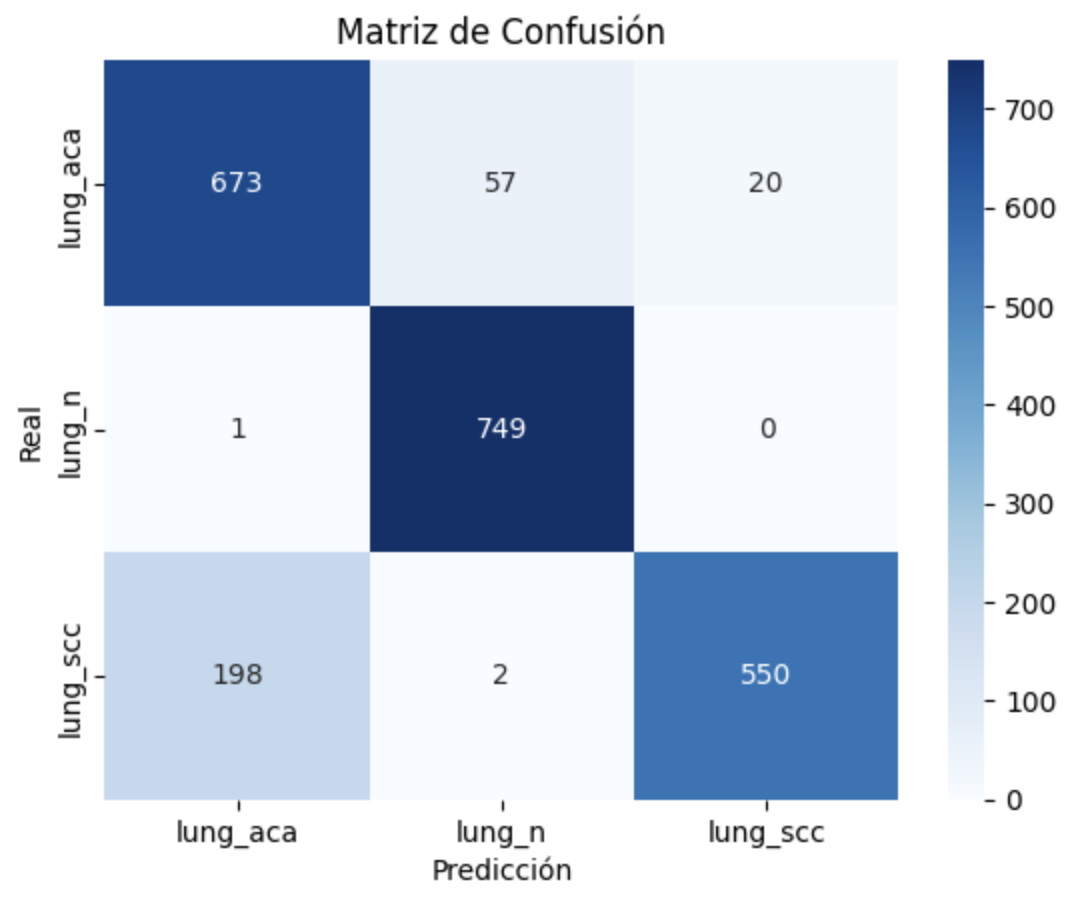
\includegraphics[width=0.45\textwidth]{figs/confusion_matrix_resnet50.png}
\caption{Matriz de confusión del modelo \textit{ResNet50}.}
\label{fig:confmatrix_resnet50}
\end{figure}

El reporte de clasificación fue el siguiente:

\begin{table}[ht]
\centering
\caption{Reporte de clasificación del modelo \textit{ResNet50} sobre el conjunto de prueba}
\begin{tabular}{|l|c|c|c|c|}
\hline
\textbf{Clase} & \textbf{Precisión} & \textbf{Recall} & \textbf{F1-score} & \textbf{Soporte} \\
\hline
lung\_aca      & 0.77 & 0.90 & 0.83 & 750 \\
lung\_n        & 0.93 & 1.00 & 0.96 & 750 \\
lung\_scc      & 0.96 & 0.73 & 0.83 & 750 \\
\hline
\textbf{Accuracy} & \multicolumn{4}{c|}{0.88 (2250 imágenes)} \\
\textbf{Macro avg} & 0.89 & 0.88 & 0.87 & 2250 \\
\textbf{Weighted avg} & 0.89 & 0.88 & 0.87 & 2250 \\
\hline
\end{tabular}
\label{tab:clasresnet50}
\end{table}



\section{Resultados y Análisis}



A pesar de que ResNet50 es una arquitectura profunda ampliamente validada en tareas generales de clasificación de imágenes, los resultados obtenidos en este trabajo muestran que no necesariamente supera a modelos más ligeros cuando se trata de dominios visuales específicos como la histopatología.

El modelo ResNetLung (basado en ResNet-18), entrenado desde cero, logró una precisión del 96 %, superior al 88.6 % alcanzado por ResNet50. Más allá del rendimiento numérico, esta diferencia se entiende mejor al analizar la naturaleza del dataset.

En imágenes histopatológicas, especialmente aquellas teñidas con hematoxilina y eosina (H&E), las estructuras relevantes —como núcleos celulares, espacios alveolares y agrupaciones anómalas— suelen presentarse como configuraciones visuales simples: formas circulares, texturas lineales, repeticiones de puntos o agrupamientos densos. Estos patrones son visualmente distintivos, pero no excesivamente complejos, por lo que no requieren modelos con una gran profundidad ni una jerarquía de abstracciones tan pronunciada como en tareas como clasificación de escenas, objetos naturales o rostros.

En este contexto, una red liviana pero especializada puede aprender eficientemente los patrones morfológicos clave sin sobreajustarse, especialmente si se entrena desde cero sobre el dominio específico. Esto contrasta con ResNet50, cuyo preentrenamiento sobre ImageNet incorpora una fuerte inductiva visual generalista, no necesariamente alineada con las características de tejido tumoral.

Además, ResNetLung convergió en solo 10 épocas, mostrando un entrenamiento estable, sin signos de sobreajuste y con gran generalización. En cambio, ResNet50 requirió 30 épocas para aproximarse a una precisión menor, y presentó más fluctuaciones en su curva de validación, lo que indica menor estabilidad en este dominio.

Por lo que concluimos que, para datasets histológicos con estructuras visuales poco intrincadas pero altamente discriminativas, la clave no está en la complejidad del modelo, sino en su adaptación al dominio. Arquitecturas livianas bien diseñadas no solo son más eficientes computacionalmente, sino que pueden superar a modelos pesados si se alinean con la naturaleza de los datos.

\begin{table}[H]
\centering
\caption{Comparación de desempeño entre ResNetLung y ResNet50}
\label{tab:comparison}
\begin{tabular}{|l|c|c|}
\hline
\textbf{Métrica} & \textbf{ResNetLung (ResNet-18)} & \textbf{ResNet50} \\
\hline
Épocas de entrenamiento & 10 & 30 \\
Precisión general & \textbf{96.0\%} & 88.6\% \\
F1-score (macro promedio) & \textbf{0.96} & 0.87 \\
Tamaño del modelo & Bajo & Alto \\
Convergencia rápida & Sí & No \\
Tendencia al sobreajuste & Baja & Media \\
Alineación con el dominio & Alta & Moderada \\
\hline
\end{tabular}
\end{table}
\section{Conclusiones}

Los resultados obtenidos en este estudio demuestran que una arquitectura residual ligera como \textit{ResNetLung} (basada en ResNet-18) puede alcanzar un desempeño sobresaliente en la clasificación de imágenes histopatológicas pulmonares, logrando una precisión del 96\% y un macro F1-score de 0.96 tras solo 10 épocas de entrenamiento.

En comparación, una versión más profunda como ResNet-50, entrenada durante 30 épocas, obtuvo un rendimiento inferior (88.6\% de precisión), evidenciando un menor ajuste al problema pese a su mayor capacidad. Esto sugiere que, en datasets de imágenes histológicas donde los patrones tienden a ser estructuras simples (como círculos, líneas y texturas regulares propias del tejido tisular), modelos más pequeños y eficientes pueden ser más adecuados, evitando sobreajuste y reduciendo la carga computacional.

La matriz de confusión mostró que el modelo ligero clasifica con alta precisión el tejido sano y el carcinoma escamoso, mientras que las confusiones principales se dieron entre adenocarcinoma y carcinoma escamoso, posiblemente debido a la similitud visual entre estas clases. Este hallazgo abre la posibilidad de mejorar el rendimiento mediante técnicas complementarias como el aumento de datos, mecanismos de atención o entrenamiento focalizado.

Finalmente, gracias a su bajo costo computacional, rápida convergencia y facilidad de integración, \textit{ResNetLung} representa una solución prometedora para aplicaciones clínicas asistidas por IA, siendo escalable y adaptable a otros contextos médicos con necesidades similares.

\bibliographystyle{IEEEtran}
\begin{thebibliography}{1}

\bibitem{wang2024pirads}
W. Wang et al., ``PI-RADS 3 lesion classification based on ResNet18 in T2-weighted images,'' \emph{Frontiers in Oncology}, vol. 13, 2024.

\bibitem{xu2024resnet}
Y. Xu et al., ``Deep learning model based on an improved ResNet18 for on-site diagnosis of respiratory cytological samples,'' \emph{BMC Cancer}, vol. 24, no. 1, 2024.

\bibitem{he2016resnet}
K. He, X. Zhang, S. Ren, and J. Sun, ``Deep Residual Learning for Image Recognition,'' in \emph{Proc. of CVPR}, 2016.

\bibitem{kaggleLC25000}
Kaggle, ``Lung and Colon Cancer Histopathological Images,'' [Online]. Available: \url{https://www.kaggle.com/datasets/andrewmvd/lung-and-colon-cancer-histopathological-images}

\bibitem{paszke2019pytorch}
A. Paszke et al., ``PyTorch: An Imperative Style, High-Performance Deep Learning Library,'' in \emph{NeurIPS}, 2019.

\bibitem{resnetlunganon} ``LungCancer-ResNetClassifier,'' GitHub repository, 2025. [Online]. Available: \url{https://github.com/joelibaceta/LungCancer-ResNetClassifier}

\bibitem{he2016resnet}
K. He, X. Zhang, S. Ren, and J. Sun, ``Deep Residual Learning for Image Recognition,'' in \emph{Proc. of CVPR}, 2016.

\end{thebibliography}

\end{document}